\section{Performance Evaluation}
\label{sec:Evaluation}
%\vspace{0.10in}
In order to evaluate our proposed automated deployment strategy, we start with the initial Sawtooth network with five nodes. All nodes on the Sawtooth network will include the basic Sawtooth components as shown in Fig. \ref{fig:Sawtooth_Architecture}), a Validator, REST API and set of Transaction Processors running. The first node creates and distributes the genesis block. For simplicity, the authorization type between the nodes is set to default ``trust'' option, where nodes can communicate to each other without additional authentication setup. Each node is allocated the following specifications: \textbf{Memory}: 2GB, \textbf{Processor}: 2 CPUs, \textbf{Storage}: 20GB, \textbf{Network}: NAT, \textbf{OS}: Ubuntu 16.04 LTS. To simulate the nodes and network, we are using Oracle's VirtualBox\cite{oracle-virtualbox}. 

To evaluate the scenarios described in the previous section, we have designed the following network topology (Fig. \ref{fig:peering}) with 11 nodes, where five nodes (P1-P5) connect via dynamic peering and six nodes (P6-P11) connect via static peering.

The following table describes the node details, selected peering option and the time taken by the deployment script to bring the node up in order to successfully join the Blockchain network. Once the genesis node is up and running, the remaining nodes can be deployed in parallel in the case of dynamic peering, and sequential in case of static peering. The following table contains the results from a sequential deployment. 

\begin{table}[h]
\centering
\label{tab:node_details_dep}
\begin{tabular}{|l|l|l|l|l|}
\hline
Node       & IP        & Peering & Peer/Seed & Deployment Time \\ \hline
P1-Genesis & 10.0.1.10 & Dynamic & 10.0.1.10 & 2min 42sec.  \\ \hline
P2         & 10.0.1.11 & Dynamic & 10.0.1.10 & 2min 50sec.  \\ \hline
P3         & 10.0.1.12 & Dynamic & 10.0.1.10 & 3min         \\ \hline
P4         & 10.0.1.13 & Dynamic & 10.0.1.10 & 2min 35sec.  \\ \hline
P5         & 10.0.1.14 & Dynamic & 10.0.1.10 & 2min 57sec.  \\ \hline
P6         & 10.0.1.15 & Static  & 10.0.1.10 & 3min 05sec.  \\ \hline
P7         & 10.0.1.16 & Static  & 10.0.1.11 & 3min 10sec.  \\ \hline
P8         & 10.0.1.17 & Static  & 10.0.1.12 & 2min 44sec.  \\ \hline
P9         & 10.0.1.18 & Static  & 10.0.1.13 & 2min 59sec.  \\ \hline
P10        & 10.0.1.19 & Static  & 10.0.1.14 & 3min 15sec.  \\ \hline
P11        & 10.0.1.20 & Static  & 10.0.1.19 & 3min 20sec.  \\ \hline
\end{tabular}
\caption{Node details and deployment time.}
\vspace{-4mm}
\end{table}

The total time taken in case of a sequential deployment is 32 minutes and 37 seconds and the average time taken by each node is 2 minutes and 57 seconds. Moreover, the deployment time mainly depends on two more factors, the node’s processing capabilities (as described in the architecture section) and the available internet speed, which in our case on an average at the time of experiment was 85 Mbps down and 85 Mbps up.

In case of known and unknown genesis, regardless of static or dynamic peering modes selected, once all nodes are up and running, the latest transactions from each of the nodes are synchronized on all other peers of the Blockchain network. We are experimenting with a few basic transactions on different nodes and verifying the same on all other nodes. Since the transactions are very small, they are reflected immediately.

\begin{figure}[H] % H for place here
    \centering
    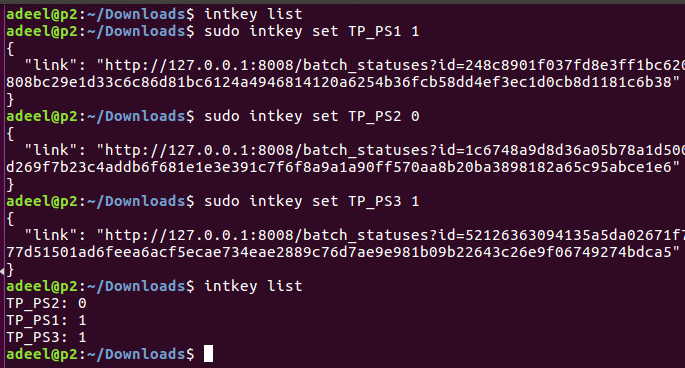
\includegraphics[scale=.60]{figs/1TP_Trans.PNG}
    \setlength{\belowcaptionskip}{-15pt}
    \caption{Transactions (Parking Sensors Data) from Traffic and Police Department on P2}
    \label{fig:p1} %refer the figure with this label
\end{figure}

\begin{figure}[H] % H for place here
    \centering
    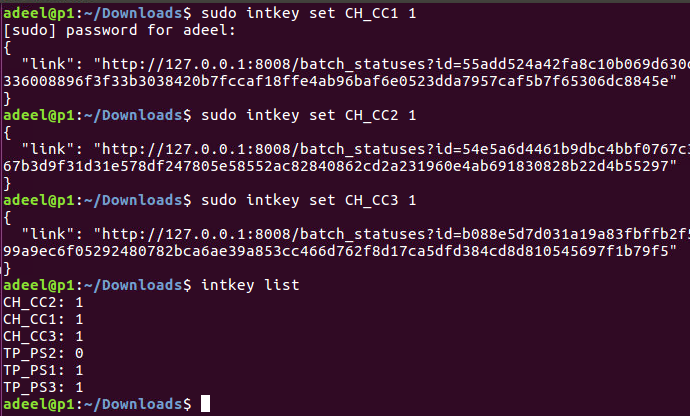
\includegraphics[scale=.60]{figs/2CQ_Trans.PNG}
    \setlength{\belowcaptionskip}{-15pt}
    \caption{Transactions (City HQ CCTV Data) from City HQ on P1}
    \label{fig:p2} %refer the figure with this label
\end{figure}

We use intkey command to create sample IntegerKey transactions. As seen in Fig. \ref{fig:p1}, the initial intkey list command returns no values. However, as we start making transactions on each client, the intkey list command starts returning newly added values. Fig. \ref{fig:p3} shows the entire intkey list synchronized on the last node.

\begin{figure}[H] % H for place here
    \centering
    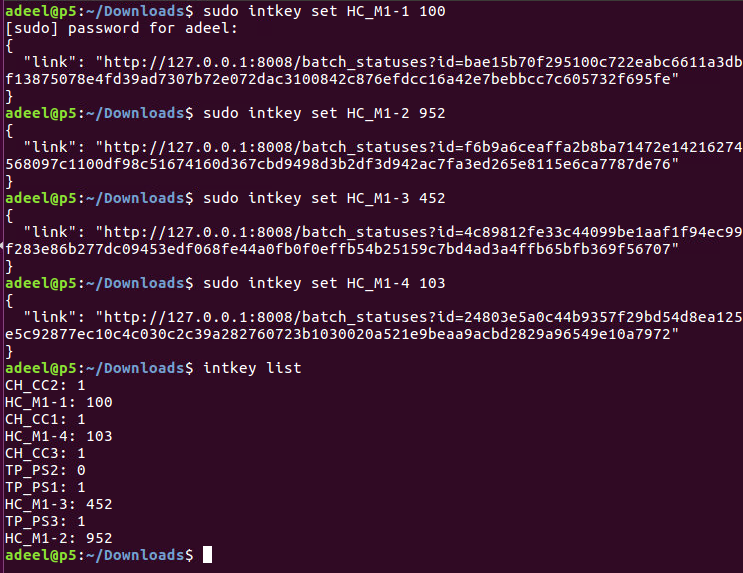
\includegraphics[scale=.50]{figs/3HC_Trans.PNG}
    \setlength{\belowcaptionskip}{-15pt}
    \caption{Transactions (Healthcare Data) from Healthcare on P5}
    \label{fig:p2} %refer the figure with this label
\end{figure}

\begin{figure}[H] % H for place here
    \centering
    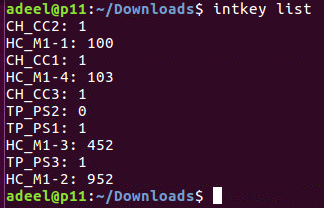
\includegraphics[scale=0.8]{figs/4P11_Trans.PNG}
    \setlength{\belowcaptionskip}{-5pt}
    \caption{Synchronized transactions from all nodes on P11}
    \label{fig:p3} %refer the figure with this label
\end{figure}

In case of the “Churning Node”, we turn off node P10 for some time. Node P10 bridges P13 with the rest of the Blockchain network. A few transactions are made during this time on the other nodes (P1-P9) and a few transactions on the isolated node P11. Peering between P11 - P10 and P10 - P5 is ``Static''. It is observed in this case that P11 is not able to transfer any transactions to the chain. While the only peer of P11 is offline and there is no other peer to agree on the transactions made by P11, those transactions are ignored and not synchronized on the chain. In the case of dynamic peering, there has to be at least one more peer actively running apart from the peer making the transaction to add the transactions to the chain. After P10 comes back online, it fetches the latest updates from its peer P5. However, P11's components need to be restarted for P11 to fetch the latest updates from P10. 

If P5 is down, isolating P10 and P11 from the rest of the network, the transactions made on either side of the network will only synchronize on both sides when P5 is connected dynamically or statically on both sides of the network in order to fetch and synchronize the updates from both sides. It is also observed that failure of the bootstrapping node or any other validator node does not halt the normal ledger operations as long as there is at least one active node aside from the node trying to add transactions to the chain. The network topology has to be designed in such a way that each node must have a backup static or dynamic peer in place so that if one goes offline, the node can communicate with the rest of the network through the other peer. Dynamic peering creates a mesh network between the nodes and peers can fetch/transmit details from other nodes on the network.
